\chapter{An Overview of Computational Solid Mechanics} \label{ch:solid_mechanics}
%
This chapter addresses some of the essential aspects of numerical approximation methods for modeling solid continua. The discussion herein will focus on the mathematical foundations of solid mechanics, beginning with the kinematics of motion and some common forms of constitutive relationships, followed by the expressions for conservation of momentum in both strong and weak form, and concluding with an analysis of the standard numerical methods utilized to solve these equations in an approximate sense. In the course of our discussion, we will make explicit the ensuing requirements placed upon any prospective approximation scheme. This will aid our analysis in subsequent chapters, and hopefully justify particular choices made in the construction of partitioned element methods.

The reader already familiar with nonlinear solid mechanics and traditional finite element methods is encouraged to proceed onward to chapter \ref{ch:pem}.

\newpage

\section{The Lagrangian Description of Motion}

Consider a body $\mathcal{B}_0 \subset \mathbb{R}^d$ consisting of a set of material points whose positions in some reference configuration at time $t = 0$ are denoted $\bm{X}$. At a later time $t > 0$, the body occupies a new configuration $\raisebox{\depth}{$\chi$} (\mathcal{B}_0, t) = \mathcal{B}_t \subset \mathbb{R}^d$, such that the motion of individual material points yields new spatial positions $\bm{x} (t)$ according to the bijection $\raisebox{\depth}{$\chi$}_t \, \colon \bm{X} \leftrightarrow \bm{x}$, i.e.
\begin{equation}
  \bm{x} = \raisebox{\depth}{$\chi$} (\bm{X}, t), \quad \bm{X} = \raisebox{\depth}{$\chi$}^{-1} (\bm{x}, t).
\end{equation}
The displacement $\bm{u} (t)$ of a given material point may be expressed as $\bm{u} = \bm{x} - \bm{X}$, and its corresponding velocity is denoted $\bm{v} (t) = \dot{\bm{x}} = \partial \bm{x} / \partial t$. Figure \ref{fig:kinematics} provides a visual interpretation of the situation described.
\begin{figure}[!h]
  \centering
  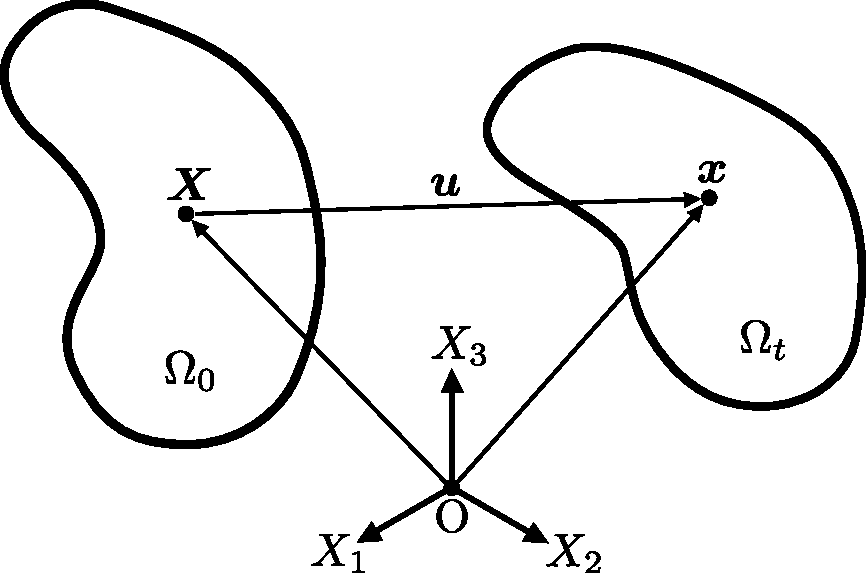
\includegraphics[width=4.0in]{figures/kinematics.pdf}
  \caption{A depiction of the motion of material points in a body $\Omega$ at time $t$.}
  \label{fig:kinematics}
\end{figure}

At a given time $t$, the Jacobian of the deformation mapping $\raisebox{\depth}{$\chi$}_t$ yields the deformation gradient $\bm{F} (t) = \nabla_X \bm{x}$ (a rank-2 tensor), defined as
\begin{equation}
  \bm{F} = \frac{\partial \bm{x}}{\partial \bm{X}} = \bm{1} + \nabla_X \bm{u},
\end{equation}
where $\nabla_X$ denotes the gradient with respect to $\bm{X}$. The deformation gradient may be used to map differential line segments $\mathrm d \bm{X}$, surface areas $\mathrm d \bm{A}$, and volumes $\mathrm d V$ defined in the reference configuration into their corresponding transformed quantities at time $t$:
\begin{equation}
  \mathrm d \bm{x}(t) = \bm{F} \, \mathrm d \bm{X}, \quad \mathrm d \bm{a}(t) = J \bm{F}^{-\mathrm T} \, \mathrm d \bm{A}, \quad \mathrm d v(t) = J \, \mathrm d V,
\end{equation}
where $J(t) \equiv \det{\bm{F}}$.

In like fashion, the spatial velocity gradient $\bm{L} (t) = \nabla_x \bm{v}$ (where $\nabla_x(t)$ denotes the gradient with respect to $\bm{x}$) may be expressed as
\begin{equation}
  \bm{L} = \frac{\partial \bm{v}}{\partial \bm{x}} = \frac{\partial \dot{\bm{x}}}{\partial \bm{X}} \frac{\partial \bm{X}}{\partial \bm{x}} = \dot{\bm{F}} \bm{F}^{-1},
\end{equation}
which may be further decomposed into a symmetric part $\bm{D}(t)$ (the rate of deformation tensor) and an anti-symmetric part $\bm{W}(t)$ (the vorticity tensor):
\begin{equation}
  \bm{D} = \frac{1}{2} (\bm{L} + \bm{L}^{\mathrm T}), \quad \bm{W} = \frac{1}{2} (\bm{L} - \bm{L}^{\mathrm T}).
\end{equation}

\subsection*{Compatibility}

Compatibility refers to the idea that a given body remains a contiguous medium following some deformation described by $\raisebox{\depth}{$\chi$}_t$. In other words, $\raisebox{\depth}{$\chi$}_t$ must characterize a continuous mapping of spatial points between different configurations in time, such that the topology of the body remains unchanged. Compatibility is characterized by the following necessary and sufficient conditions:
\begin{equation}
  \nabla_X \times \bm{F} = \bm{0} \quad \forall \bm{X} \in \mathcal{B}_0, \, t \geq 0.
  \label{eq:compatibility}
\end{equation}
Satisfaction of the above compatibility condition implies that there exists a continuous, single-valued displacement field which gives rise to the deformation characterized by $\bm{F}$.

\subsection*{Finite Strain Measures}

Consider the set of all material line segments $\mathrm d \bm{X}$ which lie in a small neighborhood around a given material point $\bm{X}$. Also, consider these same material line segments $\mathrm d \bm{x}(t)$ in the current configuration of the body after some deformation corresponding to $\bm{F} (\bm{X}, t)$ has taken place, such that $\mathrm d \bm{x} = \bm{F} \, \mathrm d \bm{X}$.

At a given material point $\bm{X}$, the deformation gradient $\bm{F} (\bm{X}, t)$ is a linear operator, which may be decomposed into two step-wise operations: a stretching operation $\bm{U}(t)$ (or $\bm{V}(t)$), and a rotation $\bm{R}(t)$, yielding the polar decomposition of $\bm{F}$:
\begin{equation}
  \bm{F} = \bm{R} \bm{U} = \bm{V} \bm{R},
\end{equation}
where $\bm{U}$ is termed the right stretch tensor, and $\bm{V}$ is the left stretch tensor. There arise from $\bm{U}$ and $\bm{V}$ two primary deformation measures: the right Cauchy-Green deformation tensor $\bm{C}(t) = \bm{U}^2$, and the left Cauchy-Green deformation tensor $\bm{B}(t) = \bm{V}^2$. Each of these, in turn, yield the two most commonly utilized finite strain measures: the Green-Lagrangian strain tensor $\bm{E}(t) = \frac{1}{2} (\bm{C} - \bm{I})$, and the Eulerian-Almansi strain tensor $\bm{e}(t) = \frac{1}{2} (\bm{I} - \bm{B}^{-1})$. It is not difficult to show that both of these strain measures reduce to the small strain tensor $\boldsymbol{\varepsilon}(t) = \frac{1}{2} (\nabla_X \bm{u} + (\nabla_X \bm{u})^{\mathrm T})$ if the displacements are sufficiently small.

Another finite strain measure that has gained attention in more recent years is the Hencky (logarithmic, or ``true'') strain tensor $\bm{H}(t) = \frac{1}{2} \log \bm{B}$. Because the Hencky strain tensor belongs to the Seth-Hill family of strain measures (as do the Green-Lagrangian and Eulerian-Almansi strain tensors), it likewise is seen to reduce to the small strain tensor in the limit of small displacements.

\section{Conservation of Linear and Angular Momentum}

For a given material body $\mathcal{B}_t \subset \mathbb{R}^d$, any open subset $\Omega_t \subset \mathcal{B}_t$ must satisfy Newton's second law of motion, such that the net external force that acts upon $\Omega_t$ is equal to the total change in linear momentum of the system, i.e.
\begin{equation}
  \frac{\mathrm d}{\mathrm dt} \int_{\Omega_t} \rho \bm{v} \, \mathrm dv = \int_{\Omega_t} \rho \bm{b} \, \mathrm dv + \int_{\partial \Omega_t} \bm{t} \, \mathrm da \quad \forall \Omega_t \subset \mathcal{B}, \, t \geq 0,
\end{equation}
where $\rho(t)$ is the mass density of the material, $\bm{v}(t)$ is the velocity field, $\bm{b}(t)$ is an applied body force per unit of mass, and $\bm{t}(t)$ is the traction vector -- a force per unit of area -- which acts on $\partial \Omega_t$ (the boundary of $\Omega_t$). Via the Cauchy tetrahedron argument, it is possible to express the traction vector $\bm{t} (\bm{n})$ as a linear function of the unit vector $\bm{n}(t)$, which is normal to the surface upon which the traction acts:
\begin{equation}
  \bm{t} = \bm{n} \cdot \boldsymbol{\sigma},
\end{equation}
where $\boldsymbol{\sigma}(t)$ is referred to as the Cauchy stress tensor. Invoking the divergence theorem, we may utilize the above relation to convert the traction boundary integral into a volume integral over $\Omega_t$:
\begin{equation}
  \int_{\partial \Omega_t} \bm{t} \, \mathrm da = \int_{\partial \Omega_t} \bm{n} \cdot \boldsymbol{\sigma} \, \mathrm da = \int_{\Omega_t} \nabla_x \cdot \boldsymbol{\sigma} \, \mathrm dv.
\end{equation}
Moreover, utilizing Reynolds' transport theorem, conservation of mass, and a change of variables in $\bm{x}$ and $\bm{X}$, it is possible to show that
\begin{equation}
  \frac{\mathrm d}{\mathrm dt} \int_{\Omega_t} \rho \bm{v} \, \mathrm dv = \int_{\Omega_t} \rho \frac{\mathrm d \bm{v}}{\mathrm dt} \, \mathrm dv,
\end{equation}
which ultimately yields
\begin{equation}
  \int_{\Omega_t} \left[ \rho (\bm{b} - \dot{\bm{v}}) + \nabla_x \cdot \boldsymbol{\sigma} \right] \, \mathrm dv = \bm{0} \quad \forall \Omega_t \subset \mathcal{B}.
\end{equation}
Since we have imposed no limitations on the choice of subset $\Omega_t$, we may invoke the localization theorem to determine a point-wise statement of momentum conservation in the body $\mathcal{B}_t$:
\begin{equation}
  \rho (\bm{b} - \dot{\bm{v}}) + \nabla_x \cdot \boldsymbol{\sigma} = \bm{0} \quad \forall \bm{x} \in \mathcal{B}_t, \, t \geq 0.
\end{equation}

Similarly, by formulating an expression for the conservation of angular momentum, we obtain an additional point-wise requirement on the symmetry of the Cauchy stress tensor:
\begin{equation}
  \boldsymbol{\sigma} = \boldsymbol{\sigma}^{\mathrm T} \quad \forall \bm{x} \in \mathcal{B}_t, \, t \geq 0.
\end{equation}

\subsection*{Measures of Stress}

As expressed earlier, the Cauchy stress tensor $\boldsymbol{\sigma}$ relates the normal $\bm{n}$ of a given surface area element $\mathrm d \bm{a} = \bm{n} \, \mathrm da$ to the corresponding force per unit of area $\bm{t}$ which acts on that surface, where the surface element $\mathrm d \bm{a}$ is defined in the current configuration of the body (at some time $t > 0$). The total force which acts on a given surface $\mathrm d \bm{a}$ is then
\begin{equation}
  \mathrm d \bm{f} = \bm{t} \, \mathrm da = \boldsymbol{\sigma}^{\mathrm T} \, \mathrm d \bm{a}.
\end{equation}
Utilizing Nanson's formula for area transformations:
\begin{equation}
  \mathrm d \bm{a} = J \bm{F}^{-\mathrm T} \, \mathrm d \bm{A},
\end{equation}
we may consider an equivalent representation of $\mathrm d \bm{f}$, such that
\begin{equation}
  \mathrm d \bm{f} = J \boldsymbol{\sigma}^{\mathrm T} \bm{F}^{-\mathrm T} \, \mathrm d \bm{A} = \bm{P} \, \mathrm d \bm{A} = \bm{p} \, \mathrm dA,
\end{equation}
where $\bm{P}(t)$ is defined as the first Piola-Kirchhoff stress tensor (which in general is not symmetric), and where $\bm{p} = \bm{N} \cdot \bm{P}^{\mathrm T}$ is the corresponding Piola traction vector, characterizing the distributed force which acts over a surface defined in the reference configuration with area $\mathrm dA$ and normal $\bm{N}$.

Another stress measure (related to the first Piola-Kirchhoff stress) is the second Piola-Kirchhoff stress tensor $\bm{S}(t)$, and is commonly defined as the pull-back of the Kirchhoff stress tensor $\boldsymbol{\tau}(t) = J \boldsymbol{\sigma}$:
\begin{equation}
  \bm{S} = \bm{F}^{-1} \boldsymbol{\tau} \bm{F}^{-\mathrm T}.
\end{equation}

\section{Constitutive Relations}

Fundamentally, we require there to be some relationship between the forces applied to a given body, and its observed deformation. Such relationships are generally referred to as constitutive models, which characterize a macroscopic connection between stress and strain in a continuum.

\subsection*{Models of Elasticity}

 Constitutive models have variable forms, mostly notably as they relate to notions of elasticity: the tendency of a material to revert to its original undeformed configuration if the applied forces are removed. Models for elastic material behavior fall into three primary categories: hyperelasticity, Cauchy-elasticity, and hypoelasticity.

Hyperelasticity is concerned with the description of a material's state through an elastic potential function, which expresses the total stored elastic strain energy $W (\bm{F})$ in the material as a function of the total deformation measured from some (nominally undeformed) reference configuration. Differentiation of this potential with respect to a given deformation measure will yield an expression for the corresponding work-conjugate measure of stress, e.g.
\begin{equation}
  \bm{P} = \frac{\partial W}{\partial \bm{F}}, \qquad \bm{S} = \frac{\partial W}{\partial \bm{E}}.
\end{equation}
Some common examples of hyperelastic models include the St. Venant-Kirchhoff material model:
\begin{equation}
  W (\bm{E}) = \frac{\lambda}{2} \text{tr} (\bm{E})^2 + \mu \, \text{tr} (\bm{E}^2),
\end{equation}
the Hencky elasticity model:
\begin{equation}
  W (\bm{H}) = \frac{\lambda}{2} \text{tr} (\bm{H})^2 + \mu \, \text{tr} (\bm{H}^2),
\end{equation}
the compressible Mooney-Rivlin solid:
\begin{equation}
  W (I_1, I_2, J) = C_{01} (J^{-4/3} I_2 - 3) + C_{10} (J^{-2/3} I_1 - 3) + D_1 (J - 1)^2,
\end{equation}
\begin{equation}
  I_1 = \text{tr} (\bm{B}), \qquad I_2 = \frac{1}{2} \left[ (\text{tr} \bm{B})^2 - \text{tr} (\bm{B}^2) \right], \qquad J = \det (\bm{F}),
\end{equation}
\begin{equation}
  D_1 = \frac{\kappa}{2}, \qquad (C_{01} + C_{10}) = \frac{\mu}{2},
\end{equation}
and the compressible Neo-Hookean solid (a special case of the Mooney-Rivlin solid where $C_{01} = 0$, and $C_1 = C_{10}$):
\begin{equation}
  W (I_1, J) = C_1 (J^{-2/3} I_1 - 3) + D_1 (J - 1)^2
\end{equation}

Cauchy-elasticity (as a terminology to describe a particular sub-class of material models) differs from hyperelasticity in the sense that the relations between particular stress and strain measures are defined directly, and do not necessarily arise from an elastic potential function. The models of linear elasticity, in particular, are generalizations of Hooke's law, namely:
\begin{equation}
  \boldsymbol{\sigma} = \bm{C} \colon \boldsymbol{\varepsilon},
\end{equation}
and are suitable for small deformations, but are typically not applicable in the context of finite deformations. By comparison, Cauchy-elastic models are defined in terms of the deformation gradient $\bm{F}$, i.e.
\begin{equation}
  \boldsymbol{\sigma} = f (\bm{F}),
\end{equation}
and are suitable in the context of finite deformations. For such models to be considered objective under a superposed rigid rotation corresponding to $\bm{R}$, they must satisfy the following condition:
\begin{equation}
  \bm{R} \boldsymbol{\sigma} \bm{R}^{\mathrm T} = f (\bm{R} \bm{F}).
\end{equation}
Such models may still suffer from being non-conservative, in the sense that the total work done by the stresses acting on a body moving through an arbitrary closed cycle of deformation does not necessarily sum to zero. For these reasons, models of hyperelasticity are generally preferred where the use of such models is deemed appropriate. Nonetheless, Cauchy elasticity models are still useful, particularly in the context of small deformations.

In contrast, hypoelasticity models define an evolution (rate) equation in terms of the current stress and the velocity gradient at a given material point, i.e.
\begin{equation}
  \dot{\boldsymbol{\sigma}} = g(\boldsymbol{\sigma}, \bm{L}).
\end{equation}
Hypoelasticity models are in general non-conservative, and moreover may not necessarily return to a state of zero stress following a closed cycle of deformation. Hypoelasticity is generally less appropriate where hyperelastic or other elastic models may be used instead. The value of hypoelasticity lies in its ability to accommodate models for plastic flow and dissipation in the material, giving rise to the common models of hypoelasto-plasticity.

One of the primary challenges of working with hypoelastic models concerns the manner in which the rate of stress transforms under superposed rigid-body rotations. These considerations have led to the formulation of co-rotational (or objective) stress rates. A multitude of such rates exist, though only a few are found to be in common usage. Most notably, the Jaumann rate of stress $\accentset{\circ}{\boldsymbol{\sigma}}$ is defined as
\begin{equation}
  \accentset{\circ}{\boldsymbol{\sigma}} = g (\boldsymbol{\sigma}, \bm{D}) = \dot{\boldsymbol{\sigma}} + \boldsymbol{\sigma} \bm{W} - \bm{W} \boldsymbol{\sigma},
\end{equation}
where $\bm{D}$ and $\bm{W}$ specify the rate of deformation and vorticity at a given material point, respectively.

%\subsection{Equations of Material State}
%
%In a continuum body $\mathcal{B}_t$, every material point $\bm{x} \in \mathcal{B}_t$ is endowed with a ``material state'' $S_t (\bm{x})$ at time $t$. In the context of Lagrangian solid mechanics, the material state $S_t = \left\{ \boldsymbol{\sigma}, \, q_{*} \right\}$ typically consists of the Cauchy stress tensor $\boldsymbol{\sigma}$, and any (possibly tensorial) internal state variables $q_{*}$ associated with the material model.
%
%In a computational setting, the analysis is usually subdivided into discrete time steps $\left\{ t_k \right\}_{k=0}^N$, and the motion of material points from time $t_k$ to $t_{k+1}$ is described by an incremental displacement field, denoted $\hat{\bm{u}} = \bm{u}_{k+1} - \bm{u}_{k}$. The deformation associated with this motion may be characterized by an incremental deformation gradient $\hat{\bm{F}} = \partial \bm{x}_{k+1} / \partial \bm{x}_k = \bm{1} + \nabla_{x_k} \hat{\bm{u}}$.
%
%Assuming that the material behaves in a rate-independent manner, a generic constitutive model $f \colon (S_k, \nabla_{x_k} \hat{\bm{u}}) \mapsto S_{k+1}$ should yield the updated material state $S_{k+1}$ at time $t_{k+1}$ as a function of the material state $S_k$ at time $t_k$, and the incremental displacement gradient $\nabla_{x_k} \hat{\bm{u}}$.

\section{Model Boundary Value Problem}

Up to this point, we have discussed only the essential relationships which exist between physical quantities of interest in the context of solid mechanics. Ultimately, however, we should like to determine the anticipated motion and deformation of a particular body under the action of pre-determined externally applied forces. To this end, we must turn our attention to the definition -- and solution -- of boundary value problems (BVPs). Such problems must be well-posed, in the sense that there exists a unique solution to the stated problem, thereby imposing certain restrictions on the choice of boundary conditions.

\subsection*{The Strong Form Statement of Equilibrium} \label{sec:strongform}

In the context of solid mechanics, the solution of a given boundary value problem entails a complete description of the primary field variable(s). In the semi-discrete case, this refers primarily to the displacement field $\bm{u} (\bm{X},t_n)$ at all locations $\bm{X} \in \mathcal{B}_0$, and at all discrete times $\left\{ t_n \right\}_{n=0}^{N_{\mathrm t}}$ beginning at $t_0 = 0$. Under the requirements of compatibility, we presume that the displacement field is a spatially continuous function, whose derivatives up to second order are defined everywhere, i.e. $\bm{u} \in \left[ C^2 (\mathcal{B}_0) \right]^d$.

Let us examine a quasi-static solid mechanics model problem of the following form: consider an open domain $\mathcal{B}_0 \subset \mathbb{R}^d$ whose boundary $\partial \mathcal{B}_0$ consists of the partition $\left\{ \Gamma^{\mathrm D}_0, \Gamma^{\mathrm N}_0 \right\}$. Let $\bm{u} = \bar{\bm{u}}(t) \, \, \forall \bm{X} \in \Gamma^{\mathrm D}_0$ constitute a prescribed Dirichlet boundary condition imposed upon the displacement field, and $\bm{n} \cdot \boldsymbol{\sigma} = \bar{\bm{t}}(t) \, \, \forall \bm{X} \in \Gamma^{\mathrm N}_0$ be a Neumann boundary condition imposed upon the surface traction. Additionally, let us suppose that an applied body force $\bm{b}(t)$ acts upon all points $\bm{X} \in \mathcal{B}_0$. For every $t \in \left\{ t_n \right\}_{n=0}^{N_{\mathrm t}}$, we should like to determine the displacement field $\bm{u} (t) \in \mathcal{S} = \left\{ \bm{u} \in \left[ C^2 (\mathcal{B}_0) \right]^d \colon \bm{u} = \bar{\bm{u}} \, \, \forall \bm{x} \in \Gamma^{\mathrm D}_0 \right\}$ which satisfies the equations of equilibrium in a point-wise sense:
\begin{equation}
  \rho \bm{b} + \nabla_x \cdot \boldsymbol{\sigma} = \bm{0} \quad \forall \bm{x} \in \mathcal{B}_{t},
\end{equation}
and where we suppose that a constitutive model has been defined in order to relate some measure of the deformation (e.g. $\bm{F} = \bm{1} + \nabla_X \bm{u}$) to the stress (e.g. $\boldsymbol{\sigma} = f (\bm{F})$). Equivalently, we may write the equations of equilibrium in terms of quantities related to the reference configuration of the body:
\begin{equation}
  \rho_0 \bm{b} + \nabla_X \cdot \bm{P}^{\mathrm T} = \bm{0} \quad \forall \bm{X} \in \mathcal{B}_0,
\end{equation}
where $\rho_0 = J \rho$ is the mass density of the material at time $t = 0$. The above statement is commonly referred to as the ``strong form'' of the model problem, given that it requires point-wise satisfaction of equilibrium.

It should be emphasized that the Dirichlet boundary conditions and the requirements of compatibility are satisfied implicitly, as a consequence of the deliberate choice of function space $\mathcal{S}$ for the displacement field. Such functions $\bm{u} \in \mathcal{S}$ are termed ``admissible,'' as potential solutions to the boundary value problem at hand.

\subsection*{The Equivalent Weak Form Statement of Equilibrium}

In general, solutions to the strong form problem are not easily obtained. For this reason, it proves to be much more convenient to work with the (equivalent) ``weak form'' statement of the boundary value problem:

For every $t \in \left\{ t_n \right\}_{n=0}^{N_{\mathrm t}}$, find $\bm{u}(t) \in \mathcal{S} = \left\{ \bm{u} \in \left[H^{1} (\mathcal{B}_0)\right]^d \colon \bm{u} = \bar{\bm{u}} \, \, \forall \bm{X} \in \Gamma^{\mathrm D}_0 \right\}$ such that
\begin{equation}
  \mathcal{R}(\bm{u}, \bm{v}) = \int_{\mathcal{B}_t} \rho \bm{b} \cdot \bm{v} \, \mathrm dv + \int_{\Gamma^{\mathrm N}_t} \bar{\bm{t}} \cdot \bm{v} \, \mathrm da - \int_{\mathcal{B}_t} \boldsymbol{\sigma} \colon \nabla_x \bm{v} \, \mathrm dv = 0 \quad \forall \bm{v} \in \mathcal{V},
  \label{eq:weakeulerian}
\end{equation}
or equivalently
\begin{equation}
  \mathcal{R}(\bm{u}, \bm{v}) = \int_{\mathcal{B}_0} \rho_0 \bm{b} \cdot \bm{v} \, \mathrm dV + \int_{\Gamma^{\mathrm N}_0} \bar{\bm{p}} \cdot \bm{v} \, \mathrm dA - \int_{\mathcal{B}_0} \bm{P} \colon \nabla_X \bm{v} \, \mathrm dV = 0 \quad \forall \bm{v} \in \mathcal{V},
  \label{eq:weaklagrangian}
\end{equation}
where $\mathcal{V} = \left\{ \bm{v} \in \left[H^{1} (\mathcal{B}_0)\right]^d \colon \bm{v} = \bm{0} \, \, \forall \bm{X} \in \Gamma^{\mathrm D}_0 \right\}$, and
\begin{equation}
  H^{1} (\mathcal{B}_0) = \left\{ u \in L^2 (\mathcal{B}_0), \, D^{\alpha} u \in L^2 (\mathcal{B}_0) \, \, \forall | \alpha | \leq 1 \right\}.
\end{equation}

It should be remarked that the space $\mathcal{S}$ of admissible solutions to the weak form now consists of much more general functions than those considered for the strong form. In other words, the requirements on the differentiability of functions in $\mathcal{S}$ have been ``weakened.''

In (\ref{eq:weaklagrangian}), the traction boundary condition has been replaced by $\bm{p} = \bar{\bm{p}}(t) \, \, \forall \bm{X} \in \Gamma^{\mathrm N}_0$ -- i.e. a condition on the Piola (rather than Cauchy) surface traction. The function space $\mathcal{S}$ is commonly referred to as the space of admissible ``trial solutions,'' whereas $\mathcal{V}$ is called the space of ``test functions,'' and consists of all admissible variations such that $\mathcal{V} = T_{\bm{u}} \mathcal{S}$ is the tangent space to $\mathcal{S}$ (i.e. $\bm{u} + \bm{v} \in \mathcal{S} \, \, \forall \bm{u} \in \mathcal{S}, \, \bm{v} \in \mathcal{V}$). In words, our goal is determine the solution $\bm{u}$ from among all admissible trial solutions contained in $\mathcal{S}$ which satisfies equation (\ref{eq:weakeulerian}) or (\ref{eq:weaklagrangian}) for all admissible variations $\bm{v} \in \mathcal{V}$.

Under the assumptions of small displacements and linear elasticity, equations (\ref{eq:weakeulerian}) and (\ref{eq:weaklagrangian}) are equivalent, and may be more succinctly expressed in terms of a bilinear form $a \colon \mathcal{S} \times \mathcal{V} \mapsto \mathbb{R}$ and a linear form $\ell : \mathcal{V} \mapsto \mathbb{R}$ such that
\begin{equation}
  a(\bm{u}, \bm{v}) + \ell (\bm{v}) = 0 \quad \forall \bm{v} \in \mathcal{V}.
  \label{eq:bilinear_form}
\end{equation}

\section{Galerkin Approximations to the Weak Form}

In the weak form problem statement, the trial and test spaces $\mathcal{S}$ and $\mathcal{V}$ are taken to be infinite dimensional function spaces. In a practical computational setting, however, this renders the solution of such problems infeasible. Instead, most variational methods consider approximate solutions to the weak form, where $\bm{u} \in \mathcal{S}$ and $\bm{v} \in \mathcal{V}$ are replaced by $\bm{u}^h \in \mathcal{S}^h \subset \mathcal{S}$ and $\bm{v}^h \in \mathcal{V}^h \subset \mathcal{V}$, respectively. In this context, $\left\{ \varphi_a \right\}_{a = 1}^{N}$ and $\left\{ \phi_a \right\}_{a = 1}^{M}$ denote finite dimensional bases for the sub-spaces $\mathcal{S}^h$ and $\mathcal{V}^h$, such that
\begin{equation}
  \bm{u}^h (\bm{X}) = \sum_{a = 1}^N \varphi_a (\bm{X}) \bm{u}_a, \qquad \bm{v}^h (\bm{X}) = \sum_{a = 1}^M \phi_a (\bm{X}) \bm{v}_a.
\end{equation}

This yields the Galerkin approximation to the weak form:
Find $\bm{u}^h \in \mathcal{S}^h$ such that
\begin{equation}
  \mathcal{R}(\bm{u}^h, \bm{v}^h) = 0 \quad \forall \bm{v}^h \in \mathcal{V}^h,
  \label{eq:weakform}
\end{equation}
yielding the (in general, nonlinear) residual equations, in index notation:
\begin{equation}
  R_{ia} (\bm{u}^h) = \int_{\mathcal{B}_0} \rho_0 b_i \phi_a \, \mathrm dV + \int_{\Gamma^{\mathrm N}_0} \bar{p}_i \phi_a \, \mathrm dA - \int_{\mathcal{B}_0} P_{ij} \phi_{a,j} \, \mathrm dV = 0 \quad \forall i, \, a.
  \label{eq:residual}
\end{equation}

Without loss of generality, if we suppose that $\mathcal{S} = \mathcal{V}$ (provided $\bm{u} = \bm{0} \, \, \forall \bm{X} \in \Gamma^{\mathrm D}_0$), then we may select identical sub-spaces $\mathcal{S}^h = \mathcal{V}^h$ ($\left\{ \varphi_a \right\}_{a = 1}^{N} = \left\{ \phi_a \right\}_{a = 1}^{M}$), resulting in a symmetric (or Bubnov-) Galerkin method. Traditional finite element methods fall into this category. Such methods are advantageous in the sense that (for linear problems) they result in stable, symmetric bilinear forms satisfying the Galerkin orthogonality (or ``best approximation'') property -- the property that the solution error $\bm{e} = \bm{u}^h - \bm{u}$ is orthogonal to the chosen sub-space $\mathcal{S}^h$.

Petrov-Galerkin methods consider the more general case where $\mathcal{V}^h \neq \mathcal{S}^h$, resulting in differing trial and test function spaces. Such methods must guarantee satisfaction of the LBB (inf-sup) conditions to achieve convergence (these conditions are further elaborated upon at the end of this chapter.) Consequently, the selection of appropriate trial and test function spaces which result in stable discretizations is not trivial. Nonetheless, Petrov-Galerkin methods allow for greater flexibility in the construction of numerical approximation schemes.

\subsection*{Finite Element Methods}

Finite element methods (FEM) are predicated on the idea that a problem domain $\mathcal{B}_0$ can be discretized into a finite number of simpler sub-domains $\Omega_e \subset \mathcal{B}_0$, individually called elements, and collectively referred to as a ``mesh.'' The basis functions are assumed to be low-order polynomials within each element, and are compactly supported over a given patch of elements. The traditional finite element method assumes these basis functions to be $C^0$ continuous at element boundaries, yielding a priori satisfaction of compatibility.

Individual FE basis functions $\varphi_a$ are typically associated with the ``nodes'' $\bm{X}_a$ of the mesh (located at element vertices, along element edges, etc.), such that the Kronecker delta property is satisfied, i.e. $\varphi_a (\bm{X}_b) = \delta_{ab}$. Consequently, the basis functions comprise a set of interpolants for discrete values of the solution defined at the nodes.

Elements consisting of regular shapes (tetrahedra, hexahedra) also provide a natural means of effecting numerical integration of the weak form through the use of the isoparametric transformation and product Gaussian quadrature rules.

\subsection*{Consistent Linearization of the Weak Form}

	% Discuss and present a consistent linearization of the weak form
	In order to determine the solution $\bm{u}^h (t_n) \in \mathcal{S}^h$ satisfying the weak form equations at time $t_n$, the following Newton-Raphson algorithm is employed:
\begin{algorithm}
 \caption{Newton-Raphson Iteration}
 \label{alg:newtonraphson}
 	Compute initial guess $\Delta \bm{u}$ \;
	\While{$||\bm{R} (\bm{u}^h (t_{n-1})+\Delta {\bm{u}})|| < \epsilon$}{
 		Assemble $\bm{K} = \partial \bm{R} / \partial \Delta \bm{u}$ \;
 		Update $\Delta \bm{u} \leftarrow \Delta \bm{u} - \bm{K}^{-1}  \bm{R}$ \;
 	}
 	Update $\bm{u}^h (t_{n}) = \bm{u}^h (t_{n-1}) + \Delta {\bm{u}}$ \;
\end{algorithm}

	$\bm{R}$ denotes the residual (vector), and $\bm{K}$ denotes the stiffness matrix -- the Jacobian of the residual with respect to the incremental nodal displacements $\Delta \bm{u} = \bm{u}^h (t_{n}) - \bm{u}^h (t_{n-1})$. The iteration procedure is repeated until the stopping criterion $||\bm{R}|| < \epsilon$ is reached, for some specified residual measure $||\cdot||$, and tolerance $\epsilon$.
		
	Given the residual equations $R_{ia} (\bm{u}^h) = 0 \, \forall i, \, a$, we may express their first partial derivatives $\partial R_{ia} / \partial \Delta u_{jb}$ with respect to the independent unknowns $\Delta u_{jb}$ as
	\begin{equation}
	  \frac{\partial R_{ia}}{\partial \Delta u_{jb}} =
	  \int_{\Gamma^{\mathrm N}_0} \frac{\partial \bar{p}_i}{\partial \Delta u_{jb}}  \phi_a \, \mathrm dA
	 - \int_{\mathcal{B}_0} \frac{\partial P_{ik}}{\partial \Delta u_{jb}} \phi_{a,k} \, \mathrm dV,
	\end{equation}
	indicating two primary terms ($\bar{\bm{p}}$ and $\bm{P}$) which must be linearized. Subsequent discussions will focus on the linearization of the first Piola-Kirchhoff stress.
	
\subsection*{Nonlinear Deformation and Incremental Kinematics}

	Let us contemplate the linearization of $\partial P_{ik} / \partial \Delta u_{jb}$ by applying the chain-rule:
	\begin{equation}
		\frac{\partial P_{ik}}{\partial \Delta u_{jb}} = \frac{\partial P_{ik}}{\partial F_{lm}} \frac{\partial F_{lm}}{\partial \Delta u_{jb}},
	\end{equation}
	revealing the deformation ``gradient operator:''
	\begin{equation}
		\frac{\partial F_{lm}}{\partial \Delta u_{jb}} = \delta_{jl} \varphi_{b,m}.
	\end{equation}
	If an enhanced strain formulation is employed (such as the mean dilatation approach of de Souza Neto et al. \cite{Souza:96}), only the gradient operator would need to be modified; the subsequent expressions pertaining to $\partial P_{ik} / \partial F_{lm}$ would remain unchanged.

	% Present consistent linearization for finite deformations
	
	Through further application of the chain-rule, and use of the following identities:
	\begin{equation}
		\frac{\partial J}{\partial F_{lm}} = J F_{ml}^{-1}, \quad \frac{\partial F_{kj}^{-1}}{\partial F_{lm}} = F_{kl}^{-1} F_{mj}^{-1},
	\end{equation}
	one can derive the following result:
	\begin{equation}
		\frac{\partial P_{ik}}{\partial F_{lm}} = J \sigma_{ij} (F_{ml}^{-1} F_{kj}^{-1} + F_{kl}^{-1} F_{mj}^{-1})  + J \frac{\partial \sigma_{ij}}{\partial F_{lm}} F_{kj}^{-1}.
	\end{equation}
	If the material model allows for the Cauchy stress to be written directly as a function of the deformation gradient (i.e. $\boldsymbol{\sigma} = f(\bm{F})$, as is the case for Cauchy-elastic material models), then a consistent linearization for $\partial \sigma_{ij} / \partial F_{lm}$ may be obtained by direct differentiation.
	
	Otherwise (for hypoelastic material models of the form $\dot{\boldsymbol{\sigma}} = g(\boldsymbol{\sigma}, \bm{L})$), the integral of the stress rate over some finite time interval $\Delta t = t_{n} - t_{n-1}$ is required:
	\begin{equation}
		\boldsymbol{\sigma} (t_{n}) = \boldsymbol{\sigma} (t_{n-1}) + \int_{t_{n-1}}^{t_{n}} \dot{\boldsymbol{\sigma}} (\boldsymbol{\sigma}, \bm{L}) \, \mathrm dt.
		\label{eq:stress_update}
	\end{equation}
	The corresponding increment of deformation is denoted $\hat{\bm{F}} = \bm{F} (t_{n}) \bm{F}^{-1} (t_{n-1}) = \hat{\bm{R}} \hat{\bm{U}}$. In the incremental kinematics algorithm of Rashid \cite{Rashid:93}, the incremental deformation $\hat{\bm{F}}$ is applied sequentially, in two distinct steps which consist of: a constant rate of stretching $\bm{D} = \frac{1}{\Delta t} \log \hat{\bm{U}}$ with $\bm{W} = 0$, followed by an impulsive (rigid) rotation $\hat{\bm{R}}$. Following this procedure, equation (\ref{eq:stress_update}) becomes:
	\begin{equation}
		\boldsymbol{\sigma} (t_{n}) = \hat{\bm{R}} \left[ \boldsymbol{\sigma} (t_{n-1}) + \int_{t_{n-1}}^{t_{n}} \dot{\boldsymbol{\sigma}} (\boldsymbol{\sigma}, \bm{D}) \, \mathrm dt \right] \hat{\bm{R}}^{\mathrm T}.
	\end{equation}
	The resulting algorithmically consistent tangent $\partial \sigma_{ij} / \partial F_{lm}$ is computed as
	\begin{equation}
		\frac{\partial \sigma_{ij}}{\partial F_{lm}} = \frac{\partial \hat{R}_{ik}}{\partial F_{lm}} \hat{R}_{nk} \sigma_{nj} + \sigma_{in} \hat{R}_{nk} \frac{\partial \hat{R}_{jk}}{\partial F_{lm}} + \hat{R}_{ik} C_{knpq} \hat{R}_{jn} \frac{\partial D_{pq}}{\partial F_{lm}} \Delta t,
	\end{equation}
	where $C_{knpq} \equiv \partial \sigma_{kn} / \partial D_{pq}$ (the material tangent modulus) is supplied by the constitutive model.
	
	The accurate computation of $\partial \hat{R}_{ik} / \partial F_{lm}$ and $\partial D_{pq} / \partial F_{lm}$ pose several nuanced challenges, requiring expressions for tensor derivatives of tensor functions ($\log \hat{\bm{U}}$, in particular). Recently, closed form expressions for the aforementioned derivatives have been developed, which utilize the eigendecomposition of $\hat{\bm{U}}$. The relevant procedures are too complicated to discuss in sufficient detail here. A forthcoming publication that addresses precisely this subject is currently in progress \cite{kinematics_paper}.
	
%	\begin{equation}
%		\frac{\partial \hat{D}_{pq}}{\partial \hat{U}_{ij}} = \frac{1}{\Delta t} \sum_{r,s} \hat{Q}_{qr} \hat{Q}_{jr} \mathcal{H} (f, \hat{\lambda}_r, \hat{\lambda}_s) \hat{Q}_{ps} \hat{Q}_{is}; \quad f (\lambda) = \log (\lambda),
%	\end{equation}
%	\begin{equation}
%		\frac{\partial \hat{U}_{ij}}{\partial \hat{B}_{kl}} = \sum_{r,s} \hat{Q}_{jr} \hat{Q}_{lr} \mathcal{H} (g, \hat{\lambda}_r^2, \hat{\lambda}_s^2) \hat{Q}_{is} \hat{Q}_{ks}; \quad g (\lambda) = \sqrt{\lambda},
%	\end{equation}
%%	\begin{equation}
%%		\frac{\partial \hat{B}_{kj}}{\partial F_{lm}} = \frac{\partial \hat{B}_{kj}}{\partial \hat{F}_{iq}} \frac{\partial \hat{F}_{iq}}{\partial F_{lm}} = \left[ \delta_{kq} \hat{F}_{ij} + \hat{F}_{ik} \delta_{jq} \right] \delta_{il} \bar{F}^{-1}_{mq} = \bar{F}^{-1}_{mk} \hat{F}_{lj} + \hat{F}_{lk} \bar{F}^{-1}_{mj},
%%	\end{equation}
%	\begin{equation}
%		\frac{\partial \hat{B}_{kj}}{\partial F_{lm}} = F^{-1}_{mi} (\hat{F}_{ik} \hat{F}_{lj} + \hat{F}_{ij} \hat{F}_{lk}),
%	\end{equation}
%	\begin{equation}
%		\frac{\partial \hat{R}_{ik}}{\partial F_{lm}} = \delta_{il} \hat{R}_{mj} F^{-1}_{jk} - \hat{R}_{in} \frac{\partial \hat{U}_{nj}}{\partial F_{lm}} \hat{U}_{jk}^{-1},
%	\end{equation}
%	where we define
%	\begin{equation}
%		\mathcal{H} (f, x, y) \equiv \left\{ \begin{array}{cc} f'(x), & x = y \\
%		\frac{f(x) - f(y)}{x - y} & x \neq y \end{array} \right. ,
%	\end{equation}
%	and $\hat{\bm{U}} = \hat{\bm{Q}} \hat{\boldsymbol{\Lambda}} \hat{\bm{Q}}^T$ represents the eigendecomposition of $\hat{\bm{U}}$, and $\hat{\lambda}_i$ denote the corresponding eigenvalues of $\hat{\bm{U}}$.

\section{Requirements for Convergence of an Approximation Method}

Because variational methods utilize finite dimensional spaces $\mathcal{S}^h$ and $\mathcal{V}^h$, they inherently incur some error $\bm{e} = \bm{u}^h - \bm{u}$ in approximating the exact solution to the original boundary value problem. The  approximation power of a given method is typically characterized by the rate at which a specified error measure $||\bm{u}^h - \bm{u}||$ (defined on $\mathcal{S}$) decreases as the dimension $N$ of the approximation space $\mathcal{S}^h$ is systematically increased. For finite element methods, increasing the dimension $N$ of the approximation space is synonymous with refining the discretization, to the extent that a specified mesh parameter $h$ (the diameter of the largest element in the mesh) is decreased. An approximation method will therefore yield solutions $\bm{u}^h$ which converge to the exact solution $\bm{u}$, provided
\begin{equation}
	\lim_{N \rightarrow \infty} ||\bm{u}^h - \bm{u}|| = \lim_{h \rightarrow 0} ||\bm{u}^h - \bm{u}|| = 0.
\end{equation}
Further, a method whose solution error can be bounded by an estimate
\begin{equation}
	||\bm{u}^h - \bm{u}|| \leq C h^p ||\bm{u}||, \quad p > 0,
\end{equation}
will converge at a rate of order $p$.

For an approximation method to achieve convergence, several conditions must be satisfied, namely: approximability, compatibility, stability, and quadrature consistency. These conditions are summarized in the following sections.

	\subsection*{Approximability}
	
	To achieve $p^{\text{th}}$-order convergence, the approximation space $\mathcal{S}^h (\mathcal{B}_0)$ must contain $[ P^{k} (\Omega) ]^d$ (the space of vector-valued polynomial functions of maximal degree $k = p-1$ defined locally over each element domain $\Omega \subset \mathcal{B}_0$) as a subset \cite{Hughes:00}. For second-order elliptic boundary value problems (e.g. solid mechanics), convergence requires that $k \geq 1$, and therefore $p \geq 2$.
	
	This property is known as \textit{approximability}, reflecting a given method's ability to well-approximate the solution locally as a low-order polynomial. Alternatively, this condition is sometimes referred to as polynomial \textit{reproducibility}, or polynomial \textit{completeness}.

% This condition can be rationalized by the Weierstrass approximation theorem, which asserts that any smooth function can be approximated by polynomials to arbitrary precision.
	
	\subsection*{Compatibility}

	 Compatibility, in an abstract sense, imposes requirements upon the continuity of trial solutions $\bm{u}^h \in \mathcal{S}^h$. For conforming finite element methods, this condition is automatically satisfied, as the trial solution space consists of continuous functions, such that $\mathcal{S}^h \subset C^0$.

By comparison, non-conforming finite element methods admit more general functions $\bm{u}^h \in \mathcal{S}^h \not\subset C^0$. Such spaces of functions must satisfy additional weak compatibility requirements. Namely, Stummel has proposed the necessary and sufficient conditions for convergence of a non-conforming finite element method, necessitating approximability, and passage of the \textit{generalized patch test} \cite{Stummel:79}:

For a given patch $\mathcal{P} \subset \overline{\mathcal{B}}_0$ and an approximating sequence of functions $u^h \in H^m (\mathcal{B}_0)$: for every $\bm{X} \in \mathcal{P}$ there exists an open neighborhood $O$ in $\mathbb{R}^d$ such that
\begin{equation}
  \lim_{h \rightarrow 0} \sum_{\forall \Omega_e} \int_{\partial \Omega_e} v \, D^\alpha u^h|_{\Omega_e} \bm{n} \, \mathrm da = \bm{0}
\end{equation}
for all test functions $v \in C^{\infty}_0 (O)$, and $| \alpha | \leq m-1$.

	Based on Stummel's generalized patch test, Shi later proposed the F-E-M test \cite{Shi:87} as an alternative, sufficient condition for convergence. The corresponding interface condition (the F-test) requires:
	\begin{equation}
		\bigg| \int_{\Omega_a \cap \Omega_b} [\![ u^h ]\!] \, \mathrm da \bigg| \leq O(h^{d/2}) ||u^h||_{\Omega_a \cup \Omega_b} \quad \forall \Omega_a \cap \Omega_b \neq \emptyset.
	\end{equation}
	The F-test is satisfied in a ``strong'' sense if
	\begin{equation}
		\int_{\Omega_a \cap \Omega_b} [\![ u^h ]\!] \, \mathrm da = 0 \quad \forall \Omega_a \cap \Omega_b \neq \emptyset,
	\end{equation}
	i.e. if the mean jump in $u^h$ across all inter-element interfaces is zero.
	
%	Alternative presentation of compatibility
	
\subsection*{Stability}

	The LBB (inf-sup) conditions (introduced in \cite{Babuska:71}, \cite{Brezzi:74}) pertain to potentially differing choices for $\mathcal{S}^h$ and $\mathcal{V}^h$ with appropriately defined norms. For the model problem with bilinear form $a \colon \mathcal{S} \times \mathcal{V} \rightarrow \mathbb{R}$, \textit{uniqueness} of a given solution is contingent upon the inf-sup condition:
	\begin{equation}
		\inf_{\bm{u}^h \in \mathcal{S}^h} \sup_{\bm{v}^h \in 
\mathcal{V}^h} \frac{a(\bm{u}^h,\bm{v}^h)}{||\bm{u}^h|| \, ||\bm{v}^h||} > 0.
	\end{equation}
	If $a$ is symmetric and $\mathcal{S}^h = \mathcal{V}^h$, this condition is equivalent to the requirement that $a$ be elliptic (coercive):
	\begin{equation}
		a(\bm{u}^h,\bm{u}^h) \geq C_c ||\bm{u}^h||^2 \quad \forall \bm{u}^h \in \mathcal{S}^h.
	\end{equation}
	\textit{Existence} of a solution further depends upon the condition that $a$ be bounded:
	\begin{equation}
		a(\bm{u}^h,\bm{v}^h) \leq C_b ||\bm{u}^h|| \, ||\bm{v}^h|| \quad \forall \bm{u}^h \in \mathcal{S}^h, \, \bm{v}^h \in \mathcal{V}^h,
	\end{equation}
	and surjective:
	\begin{equation}
		\sup_{\bm{u}^h \in 
\mathcal{S}^h} a(\bm{u}^h,\bm{v}^h) > 0 \quad \forall \bm{v}^h \in \mathcal{V}^h.
	\end{equation}
	
%	Heuristically, these conditions require that the elements utilize sufficiently accuate quadrature rules to integrate the weak form.
	Heuristically, these conditions require that the resulting finite element stiffness matrix must be of full rank (excluding rigid body modes of deformation) \cite{Bathe:06}. For displacement-based finite elements, this necessitates both: the specification of ``well-balanced'' spaces $\mathcal{S}^h$ and $\mathcal{V}^h$, and sufficiently accurate evaluation (numerical integration) of the weak form.
	
%	Show that the inf-sup conditions can be converted into local criteria for the rank sufficiency of element-level stiffness matricies.

\subsection*{Quadrature Consistency}

Considering the variational formulation of the model boundary value problem in (\ref{eq:weaklagrangian}), if the exact solution $\bm{u} \in \mathcal{S}$ to the weak form is contained within the chosen approximation space (i.e. if $\bm{u} \in \mathcal{S}^h$), we require that $\bm{u}$ be identified as the unique solution to the Galerkin approximation in (\ref{eq:weakform}), namely:
\begin{equation}
  \mathcal{R}(\bm{u}, \bm{v}^h) = 0 \quad \forall \bm{v}^h \in \mathcal{V}^h.
\end{equation}
This property is referred to as \textit{Galerkin exactness}, and is particularly relevant to the satisfaction of finite element patch tests, which demonstrate Galerkin exactness when the exact solution is a low-order polynomial.

In particular, given a stress field $P_{ij}$ arising from the exact solution $\bm{u} \in \mathcal{S}^h$, and for the given boundary conditions $\bar{p}_i = P_{ij} N_j$ and $\rho_0 b_i = - P_{ij,j}$, we may express the residual equations as
\begin{equation}
	R_{ia} = \int_{\mathcal{B}_0} P_{ij} \phi_{a,j} \, \mathrm dV + \int_{\mathcal{B}_0} P_{ij,j} \phi_a \, \mathrm dV - \int_{\partial \mathcal{B}_0} P_{ij} N_j \phi_a \, \mathrm dA = 0 \quad \forall i, \, a.
\end{equation}
If we suppose that the exact solution is well-approximated by low-order polynomials up to order $k$, i.e.
\begin{equation}
  u_{i} (\bm{X}) = \sum_{|\alpha| = 0}^{k} a_{i\alpha} \bm{X}^\alpha, \quad P_{ij} (\bm{X}) = \sum_{|\alpha| = 0}^{k-1} b_{ij\alpha} \bm{X}^\alpha,
\end{equation}
then the resulting conditions for Galerkin exactness are:
\begin{equation}
  \int_{\mathcal{B}_0} \bm{X}^{\alpha} \phi_{a,i} \, \mathrm dV + \int_{\mathcal{B}_0} \bm{X}^{\alpha}_{,i} \phi_a \, \mathrm dV = \int_{\partial \mathcal{B}_0} \bm{X}^{\alpha} N_i \phi_a \, \mathrm dA \quad \forall i, \, a, \, | \alpha | \leq k-1,
\end{equation}
where $k \geq 1$ denotes the corresponding degree of polynomial completeness exhibited by the trial solution space. The above consistency requirements must hold over the problem domain $\mathcal{B}_0$ as a whole, or equivalently over each individual element domain $\Omega_e$:
\begin{equation}
  \int_{\Omega_e} \bm{X}^{\alpha} \phi_{a,i} \, \mathrm dV + \int_{\Omega_e} \bm{X}^{\alpha}_{,i} \phi_a \, \mathrm dV = \int_{\partial \Omega_e} \bm{X}^{\alpha} N_i \phi_a \, \mathrm dA \quad \forall i, \, a, \, | \alpha | \leq k-1, \, \Omega_e \subset \mathcal{B}_0.
  \label{eq:consistency}
\end{equation}
The above conditions are necessary for satisfaction of the Irons patch test up to $k^{\text{th}}$ order, provided $\mathcal{S}^h \supset [ P^{k} (\mathcal{B}_0) ]^d$. It should be emphasized that these conditions apply specifically to the test functions $\phi_a \in \mathcal{V}^h$. To achieve $p^{\text{th}}$-order convergence in the $L^2 (\mathcal{B}_0)$ displacement error norm, the consistency equations must hold for $k = p-1 \geq 1$.

In most practical situations, however, the integral expressions in (\ref{eq:weakform}) are evaluated only approximately; numerical quadrature rules are defined on the elements and on their boundaries, such that
\begin{equation}
  \int_{\Omega_e} f(\bm{X}) \, \mathrm dV \approx \sum_{q=1}^{N_{\mathrm q\mathrm p}} w_q f(\bm{X}_q), \quad \int_{\partial \Omega_e} f(\bm{X}) \, \mathrm dA \approx \sum_{b=1}^{N_{\mathrm b\mathrm p}} w_b f(\bm{X}_b).
\end{equation}
This yields a discrete form of (\ref{eq:consistency}), henceforth referred to as \textit{quadrature consistency}:
\begin{equation}
  \sum_{q=1}^{N_{\mathrm q\mathrm p}} w_q \left[ \bm{X}_q^{\alpha} \phi^{(q)}_{a,i} + \bm{X}^{\alpha}_{q,i} \phi^{(q)}_a \right] = \sum_{b=1}^{N_{\mathrm b\mathrm p}} w_b \bm{X}_b^{\alpha} N^{(b)}_i \phi^{(b)}_a \quad \forall i, \, a, \, | \alpha | \leq k-1, \, \Omega_e \subset \mathcal{B}_0.
  \label{eq:quadrature_consistency}
\end{equation}
These conditions effectively impose a set constraints on the accuracy of the chosen quadrature rules, and/or on the choice of test functions. Failure to satisfy the above conditions results in issues of integration error, and correspondingly, loss of convergence.

Isoparametric finite elements employing product Gauss quadrature rules satisfy quadrature consistency automatically, even for relatively low-order quadrature rules. This renders traditional finite element methods highly efficient, as a minimal number of quadrature point evaluations are required to guarantee both stability and consistency.